\documentclass{article}




\usepackage{fullpage}
\usepackage{nopageno}
\usepackage{amsmath}
\usepackage{amsfonts}
\usepackage{graphicx}
\usepackage{framed}
\usepackage{xcolor}

\definecolor{dark_red}{rgb}{0.5,0.0,0.0}
\definecolor{dark_green}{rgb}{0.0,0.5,0.0}
\definecolor{dark_blue}{rgb}{0.0,0.0,0.5}
\definecolor{blue}{rgb}{0.0,0.0,1.0}

\newcommand{\dr}[1]{\textcolor{dark_red}{#1}}
\newcommand{\dg}[1]{\textcolor{dark_green}{#1}}
\newcommand{\db}[1]{\textcolor{dark_blue}{#1}}
\newcommand{\blue}[1]{\textcolor{blue}{#1}}



\begin{document}

\section*{Vectors}

A {\bf vector} is an ordered list of numbers. The length of the list is a positive integer, and the order of the entries matters. A vector is commonly denoted by listing the entries in triangular braces:
\[\langle u_1, u_2, u_3, ..., u_n \rangle\]
However in this course, for reasons that will become clear later, vectors are often denoted by listing their entries in a column enclosed by square parenthesis. The entries are listed from top to bottom:
\[\begin{bmatrix} u_1 \\ u_2 \\ u_3 \\ \vdots \\ u_n \end{bmatrix}\]

In contrast, a {\bf scalar} is a single number.

Variables that are vectors are often denoted by using boldface letters such as \(\mathbf{u}, \mathbf{v}, \mathbf{w}, ...\) in print, but in handwriting, vectors are often denoted by placing a left-to-right arrow above the chosen symbol: \(\vec{u}, \vec{v}, \vec{w}, ...\).

%\textbf{Examples:}
%\begin{itemize}
%\item A list of bank account balances.
%\item A list of 
%\end{itemize}

The symbol \(\mathbb{R}\) denotes the set of real numbers. The set of all vectors that have a length of \(n\) will be denoted by \(\mathbb{R}^n\). 

A common convention that will be used is that if a vector variable is denoted via a boldface letter, such as \(\mathbf{u}\), then the entries of the vector will be denoted using the same letter, but not in boldface, and using subscripts that start at \(1\) and count up to the length of the vector:

\[\mathbf{u} = \begin{bmatrix} u_1 \\ u_2 \\ u_3 \\ \vdots \\ u_n \end{bmatrix} \in \mathbb{R}^n\] %\mathbb{R} \times \mathbb{R} \times \mathbb{R} \times \cdots \times \mathbb{R} = \mathbb{R}^n\]

The ``zero vector", denoted by \(\mathbf{0}\), is a vector where every entry is \(0\). There is a different zero vector for each possible number of entries, and the number of entries in the zero vector \(\mathbf{0}\) depends on context. 




\subsection*{Basic vector arithmetic}

Now will be described the most basic of vector arithmetic, addition and scalar multiplication. Given two arbitrary vectors that have the {\bf same number of entries}, 
\[\mathbf{u} = \begin{bmatrix} u_1 \\ u_2 \\ u_3 \\ \vdots \\ u_n \end{bmatrix} \quad\text{and}\quad \mathbf{v} = \begin{bmatrix} v_1 \\ v_2 \\ v_3 \\ \vdots \\ v_n \end{bmatrix}\]

the vector sum is derived by simply adding together the corresponding entries:
\[\mathbf{u} + \mathbf{v} = \begin{bmatrix} u_1 \\ u_2 \\ u_3 \\ \vdots \\ u_n \end{bmatrix} + \begin{bmatrix} v_1 \\ v_2 \\ v_3 \\ \vdots \\ v_n \end{bmatrix} = \begin{bmatrix} u_1 + v_1 \\ u_2 + v_2 \\ u_3 + v_3 \\ \vdots \\ u_n + v_n \end{bmatrix}\]

\textbf{Examples:}
\begin{itemize}
\item 
\[\begin{bmatrix} 4 \\ -5 \end{bmatrix} + \begin{bmatrix} 13 \\ 7 \end{bmatrix} = \begin{bmatrix} 4 + 13 \\ -5 + 7 \end{bmatrix} = \begin{bmatrix} 17 \\ 2 \end{bmatrix}\]
\item 
\[\begin{bmatrix} 41 \\ -23 \\ 95 \end{bmatrix} + \begin{bmatrix} -27 \\ 70 \\ -113 \end{bmatrix} = \begin{bmatrix} 41 + (-27) \\ -23 + 70 \\ 95 + (-113) \end{bmatrix} = \begin{bmatrix} 14 \\ 47 \\ -18 \end{bmatrix}\]
\item 
\[\begin{bmatrix} -7 \\ 12 \end{bmatrix} + \begin{bmatrix} 16 \\ 10 \\ -8 \end{bmatrix} = \text{undefined}\]
\end{itemize}

Next, {\bf scalar multiplication} involves the multiplication of a vector by a single scalar (single number). If \(c\) is an arbitrary scalar, then:

\[c\mathbf{u} = \mathbf{u} c = c\begin{bmatrix} u_1 \\ u_2 \\ u_3 \\ \vdots \\ u_n \end{bmatrix} = \begin{bmatrix} c u_1  \\ c u_2 \\ c u_3 \\ \vdots \\ c u_n \end{bmatrix}\]

In the same vein, the ``negative" of a vector \(\mathbf{u}\), denoted by \(-\mathbf{u}\) is the result of computing the negative of each entry:

\[-\mathbf{u} = (-1)\mathbf{u} = -\begin{bmatrix} u_1 \\ u_2 \\ u_3 \\ \vdots \\ u_n \end{bmatrix} = \begin{bmatrix} -u_1  \\ -u_2 \\ -u_3 \\ \vdots \\ -u_n \end{bmatrix}\]

The ``subtraction" of vector \(\mathbf{v}\) from \(\mathbf{u}\) is simply the addition of the negative of \(\mathbf{v}\) to \(\mathbf{u}\):
\[\mathbf{u} - \mathbf{v} = \mathbf{u} + (-\mathbf{v}) = \begin{bmatrix} u_1 - v_1 \\ u_2 - v_2 \\ u_3 - v_3 \\ \vdots \\ u_n - v_n \end{bmatrix}\]

The ``division" of vector \(\mathbf{u}\) by scalar \(c\) is simply the multiplication of \(\mathbf{u}\) by \(\frac{1}{c}\):
\[\frac{\mathbf{u}}{c} = \frac{1}{c}\mathbf{u} = \begin{bmatrix} u_1/c  \\ u_2/c \\ u_3/c \\ \vdots \\ u_n/c \end{bmatrix}\]

\textbf{Examples:}
\begin{itemize}
\item 
\[-3\begin{bmatrix} 5 \\ -6 \end{bmatrix} = \begin{bmatrix} (-3)(5) \\ (-3)(-6) \end{bmatrix} = \begin{bmatrix} -15 \\ 18 \end{bmatrix}\]
\item 
\[\begin{bmatrix} 78 \\ 5 \\ -17 \end{bmatrix} - \begin{bmatrix} 90 \\ -8 \\ 13 \end{bmatrix} = \begin{bmatrix} 78 - 90 \\ 5 - (-8) \\ -17 - 13 \end{bmatrix} = \begin{bmatrix} -12 \\ 13 \\ -30 \end{bmatrix}\]
\item 
\[\frac{\begin{bmatrix} 12 \\ -8 \end{bmatrix}}{4} = \begin{bmatrix} 12/4 \\ (-8)/4 \end{bmatrix} = \begin{bmatrix} 3 \\ -2 \end{bmatrix}\]
\end{itemize}

Given vectors \(\mathbf{u}_1, \mathbf{u}_2, \mathbf{u}_3, ..., \mathbf{u}_k \in \mathbb{R}^n\), and coefficients \(\alpha_1, \alpha_2, \alpha_3, ..., \alpha_k \in \mathbb{R}\), the {\bf linear combination} of \(\mathbf{u}_1, \mathbf{u}_2, \mathbf{u}_3, ..., \mathbf{u}_k\) using the coefficients \(\alpha_1, \alpha_2, \alpha_3, ..., \alpha_k\) is the weighted sum:
\[\alpha_1 \mathbf{u}_1 + \alpha_2 \mathbf{u}_2 + \alpha_3 \mathbf{u}_3 + \cdots + \alpha_k \mathbf{u}_k\]  
The notion of the ``linear combination" will become very important when the objective is to build an arbitrary vector from a set of ``basis vectors" using only the operations of addition and scalar multiplication.

\textbf{Examples:}
\begin{itemize}
\item If \(\mathbf{u}_1 = \begin{bmatrix} -1 \\ 7 \end{bmatrix}\), \(\mathbf{u}_2 = \begin{bmatrix} 2 \\ -3 \end{bmatrix}\), \(\alpha_1 = 3\), and \(\alpha_2 = 5\), then the linear combination formed from these vectors using the respective coefficients is:
\[\alpha_1\mathbf{u}_1 + \alpha_2\mathbf{u}_2 = 3\begin{bmatrix} -1 \\ 7 \end{bmatrix} + 5\begin{bmatrix} 2 \\ -3 \end{bmatrix} = \begin{bmatrix} -3 \\ 21 \end{bmatrix} + \begin{bmatrix} 10 \\ -15 \end{bmatrix} = \begin{bmatrix} 7 \\ 6 \end{bmatrix}\]
\item If \(\mathbf{u}_1 = \begin{bmatrix} 7 \\ 6 \\ -6 \\ 1 \end{bmatrix}\), \(\mathbf{u}_2 = \begin{bmatrix} 1 \\ -5 \\ -7 \\ -2 \end{bmatrix}\), \(\alpha_1 = 4\), and \(\alpha_2 = -1\), then the linear combination formed from these vectors using the respective coefficients is:
\[\alpha_1\mathbf{u}_1 + \alpha_2\mathbf{u}_2 = 4\begin{bmatrix} 7 \\ 6 \\ -6 \\ 1 \end{bmatrix} - \begin{bmatrix} 1 \\ -5 \\ -7 \\ -2 \end{bmatrix}
= \begin{bmatrix} 28 \\ 24 \\ -24 \\ 4 \end{bmatrix} + \begin{bmatrix} -1 \\ 5 \\ 7 \\ 2 \end{bmatrix}
= \begin{bmatrix} 27 \\ 29 \\ -17 \\ 6 \end{bmatrix}\]
\item If \(\mathbf{u}_1 = \begin{bmatrix} 7 \\ -10 \\ 4 \end{bmatrix}\), \(\mathbf{u}_2 = \begin{bmatrix} 0 \\ -1 \\ 13 \end{bmatrix}\), \(\mathbf{u}_3 = \begin{bmatrix} -6 \\ 8 \\ -2 \end{bmatrix}\), \(\alpha_1 = -2\), \(\alpha_2 = 1\), and \(\alpha_3 = -\frac{1}{2}\), then the linear combination formed from these vectors using the respective coefficients is:
\begin{align*}
& \alpha_1\mathbf{u}_1 + \alpha_2\mathbf{u}_2 + \alpha_3\mathbf{u}_3 
= -2\begin{bmatrix} 7 \\ -10 \\ 4 \end{bmatrix} + \begin{bmatrix} 0 \\ -1 \\ 13 \end{bmatrix} - \frac{1}{2}\begin{bmatrix} -6 \\ 8 \\ -2 \end{bmatrix} 
= \begin{bmatrix} -14 \\ 20 \\ -8 \end{bmatrix} + \begin{bmatrix} 0 \\ -1 \\ 13 \end{bmatrix} + \begin{bmatrix} 3 \\ -4 \\ 1 \end{bmatrix} 
= \begin{bmatrix} -11 \\ 15 \\ 6 \end{bmatrix}
\end{align*}
\end{itemize}



\subsection*{Magnitude and dot product}

The ``magnitude", also referred to as the ``norm", of a vector \(\mathbf{u}\) is a collective measure of the ``size" of the vector's entries. The magnitude is denoted by \(\|\mathbf{u}\|\), though the notation \(|\mathbf{u}|\) also sees use as well. {\bf The magnitude of a vector is distinct from the number of entries in the vector.} 

There are many ways in which the magnitude of a vector can be quantified. All approaches must satisfy the following properties:
\begin{itemize}
\item For all vectors \(\mathbf{u}\), the magnitude will always be nonnegative: \(\|\mathbf{u}\| \geq 0\)
\item Only the zero vector can have a magnitude of \(0\): \(\|\mathbf{u}\| = 0 \implies \mathbf{u} = \mathbf{0}\)
\item For any pair of vectors \(\mathbf{u}\) and \(\mathbf{v}\) with the same number of entries, the ``triangle inequality" holds: \(\|\mathbf{u} + \mathbf{v}\| \leq \|\mathbf{u}\| + \|\mathbf{v}\|\)
\end{itemize}

Several popular approaches to measuring the norm include:
\begin{itemize}
\item The \(L_1\) norm:
\[\left\|\begin{bmatrix} u_1 \\ u_2 \\ \vdots \\ u_n \end{bmatrix}\right\| = |u_1| + |u_2| + \dots + |u_n|\]
\item The \(L_2\) norm, also referred to as the ``Euclidean norm": 
\[\left\|\begin{bmatrix} u_1 \\ u_2 \\ \vdots \\ u_n \end{bmatrix}\right\| = \sqrt{u_1^2 + u_2^2 + \cdots + u_n^2}\]
\item The \(L_{\infty}\) norm:
\[\left\|\begin{bmatrix} u_1 \\ u_2 \\ \vdots \\ u_n \end{bmatrix}\right\| = \max(|u_1|, |u_2|, \dots, |u_n|)\]
\end{itemize}

For most applications, including this course, the {\bf \(L_2\) Euclidean norm is used}. From here on out, the norm will always be Euclidean:

\[\|\mathbf{u}\| = \left\|\begin{bmatrix} u_1 \\ u_2 \\ \vdots \\ u_n \end{bmatrix}\right\| = \sqrt{u_1^2 + u_2^2 + \cdots + u_n^2}\]

Given any scalar \(c\), the multiplication of \(\mathbf{u}\) by \(c\) changes the magnitude by a factor of \(|c|\): 
\begin{align*}
\|c\mathbf{u}\| 
= & \left\|\begin{bmatrix} c u_1 \\ c u_2 \\ \vdots \\ c u_n \end{bmatrix}\right\|
= \sqrt{(c u_1)^2 + (c u_2)^2 + \dots + (c u_n)^2}
= \sqrt{c^2(u_1^2 + u_2^2 + \dots + u_n^2)} \\
= & |c| \sqrt{u_1^2 + u_2^2 + \dots + u_n^2} 
= |c| \cdot \|\mathbf{u}\|
\end{align*}
Therefore:
\[\|c\mathbf{u}\| = |c|\cdot\|\mathbf{u}\|\]

Given an arbitrary vector \(\mathbf{u}\), the vector \(\frac{\mathbf{u}}{\|\mathbf{u}\|}\) has a magnitude of \(1\):
\[\left\|\frac{\mathbf{u}}{\|\mathbf{u}\|}\right\| = \left\|\frac{1}{\|\mathbf{u}\|}\mathbf{u}\right\| = \left|\frac{1}{\|\mathbf{u}\|}\right|\|\mathbf{u}\| = \frac{1}{\|\mathbf{u}\|}\|\mathbf{u}\| = 1\]
The vector \(\frac{\mathbf{u}}{\|\mathbf{u}\|}\) is both a positive scalar multiple of \(\mathbf{u}\), and has length of \(1\). A vector that has a magnitude of \(1\) is referred to as a {\bf unit vector}, while \(\frac{\mathbf{u}}{\|\mathbf{u}\|}\) is often referred to as the ``normalization" of \(\mathbf{u}\).

Vector variables that denote unit vectors are often crowned with a ``hat": \(\hat{\mathbf{u}}\), \(\hat{\mathbf{v}}\), \(\hat{\mathbf{w}}\), ...

\textbf{Examples:}
\begin{itemize}
\item 
\[\left\|\begin{bmatrix} -4 \\ 1 \\ -2 \\ 2 \end{bmatrix}\right\| = \sqrt{(-4)^2 + 1^2 + (-2)^2 + 2^2} = \sqrt{16 + 1 + 4 + 4} = \sqrt{17 + 8} = \sqrt{25} = 5\]
\item 
\[\left\|\begin{bmatrix} 2 \\ 5 \\ -4 \\ 2 \end{bmatrix}\right\| = \sqrt{2^2 + 5^2 + (-4)^2 + 2^2} = \sqrt{4 + 25 + 16 + 4} = \sqrt{29 + 20} = \sqrt{49} = 7\]
\item 
The normalization of the vector \(\mathbf{u} = \begin{bmatrix} 2 \\ -1 \\ -2 \end{bmatrix}\) is done as follows: First compute the magnitude:
\[\|\mathbf{u}\| = \left\|\begin{bmatrix} 2 \\ -1 \\ -2 \end{bmatrix}\right\| = \sqrt{2^2 + (-1)^2 + (-2)^2} = \sqrt{4 + 1 + 4} = \sqrt{9} = 3\]  
Now normalize \(\mathbf{u}\):
\[\frac{\mathbf{u}}{\|\mathbf{u}\|} 
= \frac{1}{\|\mathbf{u}\|}\mathbf{u}   
= \frac{1}{3}\begin{bmatrix} 2 \\ -1 \\ -2 \end{bmatrix}
= \begin{bmatrix} 2/3 \\ -1/3 \\ -2/3 \end{bmatrix}\]
\end{itemize}

Next will be addressed the ``dot product". The ``dot product" is the only approach to multiplication that will be considered in this course. Given two vectors \(\mathbf{u}\) and \(\mathbf{v}\) with the same number of entries, the dot product, denoted by \(\mathbf{u} \bullet \mathbf{v}\), is:

\[\mathbf{u} \bullet \mathbf{v} = \begin{bmatrix} u_1 \\ u_2 \\ \vdots \\ u_n \end{bmatrix} \bullet \begin{bmatrix} v_1 \\ v_2 \\ \vdots \\ v_n \end{bmatrix} = u_1 v_1 + u_2 v_2 + \cdots + u_n v_n\]

What is the utility of the dot product? We will later discuss projections and orthogonality. 

The simple linear function 

\[f(x) = mx + c\]

can be generalized to multiple input variables:

\[f(x_1, x_2, ..., x_n) = m_1 x_1 + m_2 x_2 + \dots + m_n x_n + c\]

Using the dot product, the linear function \(f(x_1, x_2, ..., x_n)\) can be re-expressed as:

\[f(x_1, x_2, ..., x_n) = m_1 x_1 + m_2 x_2 + \dots + m_n x_n + c = \begin{bmatrix} m_1 \\ m_2 \\ \vdots \\ m_n \end{bmatrix} \bullet \begin{bmatrix} x_1 \\ x_2 \\ \vdots \\ x_n \end{bmatrix} + c = \mathbf{m} \bullet \mathbf{x} + c\]
where \(\mathbf{m} = \begin{bmatrix} m_1 \\ m_2 \\ \vdots \\ m_n \end{bmatrix}\) is the vector of coefficients, and \(\mathbf{x} = \begin{bmatrix} x_1 \\ x_2 \\ \vdots \\ x_n \end{bmatrix}\) is a vector comprised of the input parameters. The dot product can therefore be used to compute linear functions. 

The dot product distributes over addition:
\begin{align*}
\mathbf{u} \bullet (\mathbf{v} + \mathbf{w}) 
= & \begin{bmatrix} u_1 \\ u_2 \\ \vdots \\ u_n \end{bmatrix} \bullet \begin{bmatrix} v_1 + w_1 \\ v_2 + w_2 \\ \vdots \\ v_n + w_n \end{bmatrix} 
= u_1(v_1 + w_1) + u_2(v_2 + w_2) + ... + u_n(v_n + w_n) \\
= & (u_1 v_1 + u_1 w_1) + (u_2 v_2 + u_2 w_2) + ... + (u_n v_n + u_n w_n) \\
= & (u_1 v_1 + u_2 v_2 + ... + u_n v_n) + (u_1 w_1 + u_2 w_2 + ... + u_n w_n) \\
= & \mathbf{u} \bullet \mathbf{v} + \mathbf{u} \bullet \mathbf{w}
\end{align*}

Therefore:
\[\mathbf{u} \bullet (\mathbf{v} + \mathbf{w}) = \mathbf{u} \bullet \mathbf{v} + \mathbf{u} \bullet \mathbf{w}\]


The ``Cauchy-Schwartz inequality" is:
\[|\mathbf{u} \bullet \mathbf{v}| \leq \|\mathbf{u}\|\cdot\|\mathbf{v}\|\]
%\textbf{Proof:}





Lastly, the dot product can be used to compute the magnitude:

\[\|\mathbf{u}\| = \sqrt{u_1^2 + u_2^2 + \cdots + u_n^2} = \sqrt{\mathbf{u} \bullet \mathbf{u}}\]

\textbf{Examples:}
\begin{itemize}
\item 
\[\begin{bmatrix} -5 \\ 1 \\ 4 \end{bmatrix} \bullet \begin{bmatrix} -7 \\ 8 \\ -11 \end{bmatrix} = (-5)(-7) + (1)(8) + (4)(-11) = 35 + 8 - 44 = -1\]
\item The function \(f(x, y, z) = 3x + 7 - 4y + 2z\) can be re-expressed as:
\[f\left(\begin{bmatrix} x \\ y \\ z \end{bmatrix}\right) = \begin{bmatrix} 3 \\ -4 \\ 2 \end{bmatrix} \bullet \begin{bmatrix} x \\ y \\ z \end{bmatrix} + 7 \]
\end{itemize}







\section*{Vectors as displacements}

Many introductions to vectors introduce vectors as ``quantities with magnitude and direction". Vectors are commonly envisioned as arrows whose length is the magnitude, and whose direction is the vector's direction. These arrows can be positioned anywhere without affecting the vector's value, but the length and direction must be preserved. 

How do vectors, when defined as lists of numbers, connect with the geometric definition of vectors as arrows? An arrow can be quantified by listing the difference in \(x\)-coordinate between the head and tail, the difference in \(y\)-coordinate between the head and tail, and the difference in \(z\)-coordinate between the head and tail as a \(3\) element vector. 

\begin{tabular}{cc}
\parbox{0.5\textwidth}{
Given two points in space \(A\) and \(B\), the position of point \(B\) relative to point \(A\), is referred to as the {\bf displacement} of \(B\) relative to \(A\), also referred to as the displacement from \(A\) to \(B\). The displacement is often visualized as an arrow that originates at \(A\) and terminates at \(B\). The displacement of point \(B(x_2, y_2, z_2)\) relative to point \(A(x_1, y_1, z_1)\) is denoted by \(\overrightarrow{AB}\) and is:
\[\overrightarrow{AB} = \begin{bmatrix} x_2 - x_1 \\ y_2 - y_1 \\ z_2 - z_1 \end{bmatrix}\]
Given an arbitrary \(3\) element vector \(\mathbf{u} = \begin{bmatrix} u_x \\ u_y \\ u_z \end{bmatrix}\), if the coordinates of the vector arrow's tail is \((x_0, y_0, z_0)\), then the coordinates of the vector arrow's head is \((x_0 + u_x, y_0 + u_y, z_0 + u_z)\).
} & \parbox{0.5\textwidth}{
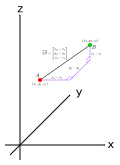
\includegraphics[width = 0.5\textwidth]{displacement_vector}
}
\end{tabular}

\textbf{Examples:}
\begin{itemize}
\item The displacement of point \(C(7, -1, 4)\) relative to point \(D(1, 0, -11)\) is:
\[\overrightarrow{DC} = \begin{bmatrix} 7 - 1 \\ (-1) - 0 \\ 4 - (-11) \end{bmatrix} = \begin{bmatrix} 6 \\ -1 \\ 15 \end{bmatrix}\]
\item The displacement from point \(X(6, -8, 7)\) to point \(Y(0, -10, 11)\) is:
\[\overrightarrow{XY} = \begin{bmatrix} 0 - 6 \\ (-10) - (-8) \\ 11 - 7 \end{bmatrix} = \begin{bmatrix} -6 \\ -2 \\ 4 \end{bmatrix}\]
\item The displacement from point \(B(9, 0, -1)\) to point \(C(12, -3, 5)\) is:
\[\overrightarrow{BC} = \begin{bmatrix} 12 - 9 \\ (-3) - 0 \\ 5 - (-1) \end{bmatrix} = \begin{bmatrix} 3 \\ -3 \\ 6 \end{bmatrix}\]
\item Given the vector \(\mathbf{u} = \begin{bmatrix} -8 \\ 5 \\ 1 \end{bmatrix}\), if the tail of the vector arrow is located at \((-2, -1, -5)\), then the head of the vector arrow is located at 
\[((-2)+(-8), (-1)+5, (-5)+1) = (-10, 4, -4)\]  
\end{itemize}

When the zero vector \(\mathbf{0}\) is envisioned as an arrow, the tail and end are the same point. The arrow has a length of \(0\), and has {\bf no direction}. 


\subsection*{Vector arrow arithmetic}

When vectors are envisioned as arrows, the sum of two vectors is performed using the head-to-tail rule. Given two arbitrary vectors \(\mathbf{u}\) and \(\mathbf{v}\), the sum \(\mathbf{u} + \mathbf{v}\) is computed by moving the arrow that represents \(\mathbf{v}\) so that its tail is the same point as the head of the arrow that represents \(\mathbf{u}\). The arrow that represents \(\mathbf{u} + \mathbf{v}\) has the tail of \(\mathbf{u}\), and the had of \(\mathbf{v}\) as seen in the image below. In the image below, there is a triangle with vertices \(A(x_1, y_1, z_1)\), \(B(x_2, y_2, z_2)\), and \(C(x_3, y_3, z_3)\). The vector \(\mathbf{u}\) is the displacement from point \(A\) to \(B\), the vector \(\mathbf{v}\) is the displacement from \(B\) to \(C\), and the vector sum \(\mathbf{u} + \mathbf{v}\) is the displacement from \(A\) to \(C\). These displacements are:

\[\mathbf{u} = \overrightarrow{AB} = \begin{bmatrix} x_2 - x_1 \\ y_2 - y_1 \\ z_2 - z_1 \end{bmatrix} \quad\text{and}\quad \mathbf{v} = \overrightarrow{BC} = \begin{bmatrix} x_3 - x_2 \\ y_3 - y_2 \\ z_3 - z_2 \end{bmatrix} \quad\text{and}\quad \mathbf{u}+\mathbf{v} = \overrightarrow{AC} = \begin{bmatrix} x_3 - x_1 \\ y_3 - y_1 \\ z_3 - z_1 \end{bmatrix}\]

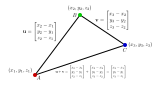
\includegraphics[width = \textwidth]{displacement_addition}


When vectors are envisioned as arrows, the multiplication of a scalar \(c\) with a vector \(\mathbf{u}\) is performed by increasing the length of \(\mathbf{u}\) by a factor of \(|c|\). If \(c\) is negative, then the direction is reversed. In the image below, there are \(3\) points in a straight line \(A\), \(B\), and \(C\). The vector \(\mathbf{u}\) is the displacement from point \(A\) to \(B\). The vector \(c\mathbf{u}\) is the displacement from point \(A\) to \(C\). The distance from \(A\) to \(C\) is \(c\) times the distance from \(A\) to \(B\), and the changes in the coordinates between the tail and head of the vector \(\overrightarrow{AB}\) are increased by a factor of \(c\) as well.

\[\mathbf{u} = \overrightarrow{AB} = \begin{bmatrix} \Delta x \\ \Delta y \\ \Delta z \end{bmatrix} \quad\text{and}\quad c\mathbf{u} = \overrightarrow{AC} = \begin{bmatrix} c\Delta x \\ c\Delta y \\ c\Delta z \end{bmatrix}\]

\begin{center}
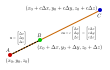
\includegraphics[width = 0.75\textwidth]{displacement_scalar_multiplication}
\end{center}


When vectors are envisioned as arrows, computing the negative of a vector simply involves reversing the orientation of the arrow. In the image below, there are two points \(A(x_1, y_1, z_1)\) and \(B(x_2, y_2, z_2)\). Vector \(\mathbf{u}\) is the displacement from point \(A\) to \(B\), and the vector \(-\mathbf{u}\) is the displacement from point \(B\) to \(A\).

\[\mathbf{u} = \overrightarrow{AB} = \begin{bmatrix} x_2 - x_1 \\ y_2 - y_1 \\ z_2 - z_1 \end{bmatrix} \quad\text{and}\quad -\mathbf{u} = \overrightarrow{BA} = \begin{bmatrix} x_1 - x_2 \\ y_1 - y_2 \\ z_1 - z_2 \end{bmatrix}\]

\begin{center}
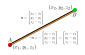
\includegraphics[width = 0.75\textwidth]{displacement_vector_negative}
\end{center}

\begin{center}
\begin{tabular}{cc}
\parbox{0.5\textwidth}{
The image to the right depicts a rectangular prism. The goal is to use linear combinations of the vectors \(\mathbf{u}\), \(\mathbf{v}\), and \(\mathbf{w}\) to express the vectors \(\mathbf{p}\), \(\mathbf{q}\), \(\mathbf{r}\), and \(\mathbf{s}\). 
\begin{itemize}
\item[*] \(\mathbf{p} = \mathbf{v} - \mathbf{u} = (-1)\mathbf{u} + (1)\mathbf{v} + (0)\mathbf{w}\)
\item[*] \(\mathbf{q} = \mathbf{w} - \mathbf{v} = (0)\mathbf{u} + (-1)\mathbf{v} + (1)\mathbf{w}\)
\item[*] \(\mathbf{r} = \mathbf{u} + \mathbf{q} = (1)\mathbf{u} + (-1)\mathbf{v} + (1)\mathbf{w}\)
\item[*] \(\mathbf{s} = \mathbf{p} + \mathbf{q} = (-1)\mathbf{u} + (0)\mathbf{v} + (1)\mathbf{w}\)
\end{itemize}
} & \parbox{0.5\textwidth}{
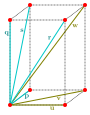
\includegraphics[width = 0.5\textwidth]{displacement_vector_lin_comb_example}
}
\end{tabular}
\end{center}


\subsection*{Parallelism}

When vectors are envisioned as arrows, two vectors \(\mathbf{u}\) and \(\mathbf{v}\) are considered to be ``parallel" if one vector is equal to the other vector multiplied by a nonzero scalar. There must exist a nonzero scalar \(c\) such that \(\mathbf{v} = c\mathbf{u}\). Consider the two nonzero vectors \(\mathbf{u} = \begin{bmatrix} u_x \\ u_y \\ u_z \end{bmatrix}\) and \(\mathbf{v} = \begin{bmatrix} v_x \\ v_y \\ v_z \end{bmatrix}\). To determine if \(\mathbf{u}\) and \(\mathbf{v}\) are parallel, the ratios between the corresponding components, \(v_x/u_x\), \(v_y/u_y\), and \(v_z/u_z\) need to be computed. Each of these ratios gives a value of \(c\). If all of these ratios are equal, then the vectors are parallel, with \(c\) being the common value. {\bf Any \(0/0\) ratio is a ``wildcard" and should be ignored.} 

\textbf{Examples:}
\begin{itemize}
%%%%%%%%%%%%%%%%%%%%
\item Given vectors \(\mathbf{u} = \begin{bmatrix} 6 \\ -2 \\ 8 \end{bmatrix}\) and \(\mathbf{v} = \begin{bmatrix} -9 \\ 3 \\ -12 \end{bmatrix}\), the ratios between the corresponding components are: 
\[v_x/u_x = -9/6 = -3/2 \quad\text{and}\quad v_y/u_y = 3/(-2) = -3/2 \quad\text{and}\quad v_z/u_z = -12/8 = -3/2\]
Since these ratios are all equal, \(\mathbf{u}\) and \(\mathbf{v}\) are {\bf parallel}.
%%%%%%%%%%%%%%%%%%%%
\item Given vectors \(\mathbf{u} = \begin{bmatrix} -3 \\ 15 \\ 6 \end{bmatrix}\) and \(\mathbf{v} = \begin{bmatrix} 7 \\ 35 \\ -14 \end{bmatrix}\), the ratios between the corresponding components are:
\[v_x/u_x = 7/(-3) = -7/3 \quad\text{and}\quad v_y/u_y = 35/15 = 7/3 \quad\text{and}\quad v_z/u_z = -14/6 = -7/3\]    
Since these ratios are not all equal, \(\mathbf{u}\) and \(\mathbf{v}\) are {\bf not parallel}.
%%%%%%%%%%%%%%%%%%%%
\item Given vectors \(\mathbf{u} = \begin{bmatrix} -18 \\ 0 \\ -27 \end{bmatrix}\) and \(\mathbf{v} = \begin{bmatrix} 10 \\ 0 \\ 15 \end{bmatrix}\), the ratios between the corresponding components are:
\[v_x/u_x = 10/(-18) = -5/9 \quad\text{and}\quad v_y/u_y = 0/0 \quad\text{and}\quad v_z/u_z = 15/(-27) = -5/9\]
The \(0/0\) reflects the fact that \(v_y = c u_y\) for any value of \(c\), and so the \(0/0\) ratio is a ``wildcard" that is ``equal" to any other ratio. The other ratios are equal so \(\mathbf{u}\) and \(\mathbf{v}\) are {\bf parallel}.
%%%%%%%%%%%%%%%%%%%%
\item Given vectors \(\mathbf{u} = \begin{bmatrix} -3 \\ 0 \\ 6 \end{bmatrix}\) and \(\mathbf{v} = \begin{bmatrix} 5 \\ 4 \\ -10 \end{bmatrix}\), the ratios between the corresponding components are:
\[v_x/u_x = 5/(-3) = -5/3 \quad\text{and}\quad v_y/u_y = 4/0 = \pm\infty \quad\text{and}\quad v_z/u_z = -10/6 = -5/3\]
Since these ratios are not all equal, \(\mathbf{u}\) and \(\mathbf{v}\) are {\bf not parallel}. In general, if one vector has a component that is \(0\), and the corresponding component is nonzero in the other vector, then it is immediately known that the vectors are not parallel.
\end{itemize}

{\bf Note that while the definition of parallelism given here requires that both vectors be nonzero, other contexts may allow for zero vectors to be parallel to nonzero vectors.}


\subsection*{Elementary basis vectors}

The ``elementary basis vectors" is a simple set of \(3\) vectors such that every vector that is a displacement in \(3\) dimensions is a linear combination of the elementary basis vectors. More specifically, the elementary basis vectors are:

\[\hat{\mathbf{i}} = \begin{bmatrix} 1 \\ 0 \\ 0 \end{bmatrix} \quad\text{and}\quad \hat{\mathbf{j}} = \begin{bmatrix} 0 \\ 1 \\ 0 \end{bmatrix} \quad\text{and}\quad \hat{\mathbf{k}} = \begin{bmatrix} 0 \\ 0\\ 1 \end{bmatrix}\]

Every vector \(\mathbf{u} = \begin{bmatrix} u_x \\ u_y \\ u_z \end{bmatrix}\) can be expressed as a linear combination of the elementary basis vectors \(\hat{\mathbf{i}}\), \(\hat{\mathbf{j}}\), and \(\hat{\mathbf{k}}\):
\[\mathbf{u} = \begin{bmatrix} u_x \\ u_y \\ u_z \end{bmatrix} = u_x \hat{\mathbf{i}} + u_y \hat{\mathbf{j}} + u_z \hat{\mathbf{k}}\]


\subsection*{Vector arrow magnitude and dot product}

When vectors are envisioned as arrows, the magnitude of the vector is the length of the arrow, which is equivalent to the Euclidean norm via the Pythagorean theorem, as demonstrated in the image below:

\begin{center}
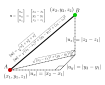
\includegraphics[width = 0.75\textwidth]{displacement_vector_magnitude}
\end{center}

\textbf{Examples:}
\begin{itemize}
\item Given the points \(A(3, 1, -4)\) and \(B(2, 4, -7)\), the displacement from \(A\) to \(B\) is \(\overrightarrow{AB} = \begin{bmatrix} 2 - 3 \\ 4 - 1 \\ (-7) - (-4) \end{bmatrix} = \begin{bmatrix} -1 \\ 3 \\ -3 \end{bmatrix}\). The distance between points \(A\) and \(B\) is the magnitude of \(\overrightarrow{AB}\) which is:
\[AB = \left\|\overrightarrow{AB}\right\| = \sqrt{(-1)^2 + 3^3 + (-3)^2} = \sqrt{1 + 9 + 9} = \sqrt{19}\]
\end{itemize}

As previously defined, a {\bf unit vector} is a vector with a magnitude of \(1\), and therefore the arrow associated with a unit vector has a length of \(1\). The normalization of a vector \(\mathbf{u}\) was previously defined as a vector that is \(\mathbf{u}\) multiplied by a positive scalar and has a magnitude of \(1\). This positive scalar is \(\frac{1}{\|\mathbf{u}\|}\), and the normalization of \(\mathbf{u}\) is \(\frac{\mathbf{u}}{\|\mathbf{u}\|}\). The normalization is an arrow that is parallel to \(\mathbf{u}\), but has a length of \(1\).

\begin{center}

\includegraphics[width = 0.75\textwidth]{displacement_vector_normalization}
\end{center}

\textbf{Examples:}
\begin{itemize}
\item The normalization of the vector \(\mathbf{u} = \begin{bmatrix} 3 \\ -1 \\ 2 \end{bmatrix}\) is done as follows: First compute the magnitude:
\[\|\mathbf{u}\| = \left\|\begin{bmatrix} 3 \\ -1 \\ 2 \end{bmatrix}\right\| = \sqrt{3^2 + (-1)^2 + 2^2} = \sqrt{9 + 1 + 4} = \sqrt{14}\]  
Now normalize \(\mathbf{u}\):
\[\frac{\mathbf{u}}{\|\mathbf{u}\|} 
= \frac{1}{\|\mathbf{u}\|}\mathbf{u}   
= \frac{1}{\sqrt{14}}\begin{bmatrix} 3 \\ -1 \\ 2 \end{bmatrix}
= \begin{bmatrix} 3/\sqrt{14} \\ -1/\sqrt{14} \\ 2/\sqrt{14} \end{bmatrix}\]
\end{itemize}

\vspace{5mm}

Now with regards to the dot product, given the two vectors \(\mathbf{u} = \begin{bmatrix} u_x \\ u_y \\ u_z \end{bmatrix}\) and \(\mathbf{v} = \begin{bmatrix} v_x \\ v_y \\ v_z \end{bmatrix}\), the dot product was defined to be \(\mathbf{u} \bullet \mathbf{v} = u_x v_x + u_y v_y + u_z v_z\). With regards to the understanding of vectors as arrows, if \(\theta\) is the angle between the arrows that represent \(\mathbf{u}\) and \(\mathbf{v}\), then 
\[\mathbf{u} \bullet \mathbf{v} = \|\mathbf{u}\|\|\mathbf{v}\|\cos\theta\]
{\bf These definitions are equivalent, and result in the same outcome.}

\begin{center}
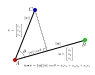
\includegraphics[width = 0.75\textwidth]{displacement_vector_dot_product}
\end{center}

The dot product is often used to compute the angle \(\theta\) between the two arrows represented by the two vectors \(\mathbf{u}\) and \(\mathbf{v}\). \(\mathbf{u} \bullet \mathbf{v} = u_x v_x + u_y v_y + u_z v_z\) is easy to compute, and:
\[\mathbf{u} \bullet \mathbf{v} = \|\mathbf{u}\|\|\mathbf{v}\|\cos\theta \iff \cos\theta = \frac{\mathbf{u} \bullet \mathbf{v}}{\|\mathbf{u}\| \|\mathbf{v}\|} \iff \theta = \cos^{-1}\left(\frac{\mathbf{u} \bullet \mathbf{v}}{\|\mathbf{u}\| \|\mathbf{v}\|}\right)\] 

Of particular interest is the scenario where \(\mathbf{u} \bullet \mathbf{v} = 0\) and \(\mathbf{u}\) and \(\mathbf{v}\) are both non-zero. In this case \(\theta = 90^\circ\), and the two vectors are said to be ``orthogonal", which is another way of saying perpendicular.

In addition, if \(\mathbf{u} \bullet \mathbf{v} > 0\), then \(\theta < 90^\circ\) so the angle between \(\mathbf{u}\) and \(\mathbf{v}\) is acute. If \(\mathbf{u} \bullet \mathbf{v} < 0\), then \(\theta > 90^\circ\) so the angle between \(\mathbf{u}\) and \(\mathbf{v}\) is obtuse.

\textbf{Examples:}
\begin{itemize}
%%%%%%%%%%%%%%%%%%%%%%%%%
\item If \(\mathbf{u} = \begin{bmatrix} -1 \\ 7 \\ 2 \end{bmatrix}\) and \(\mathbf{v} = \begin{bmatrix} 3 \\ 2 \\ 5 \end{bmatrix}\), then 
\[\mathbf{u} \bullet \mathbf{v} = (-1)(3) + (7)(2) + (2)(5) = -3 + 14 + 10 = 21\]
\[\|\mathbf{u}\| = \sqrt{(-1)^2 + 7^2 + 2^2} = \sqrt{1 + 49 + 4} = \sqrt{54}\]
\[\|\mathbf{v}\| = \sqrt{3^2 + 2^2 + 5^2} = \sqrt{9 + 4 + 25} = \sqrt{38}\]
\[\theta = \cos^{-1}\left(\frac{\mathbf{u} \bullet \mathbf{v}}{\|\mathbf{u}\| \|\mathbf{v}\|}\right) = \cos^{-1}\left(\frac{21}{(\sqrt{54})(\sqrt{38})}\right) \approx 62.3812^\circ\]
%%%%%%%%%%%%%%%%%%%%%%%%%
\item If \(\mathbf{u} = \begin{bmatrix} 5 \\ -2 \\ -1 \end{bmatrix}\) and \(\mathbf{v} = \begin{bmatrix} -3 \\ -10 \\ 5 \end{bmatrix}\), then 
\[\mathbf{u} \bullet \mathbf{v} = (5)(-3) + (-2)(-10) + (-1)(5) = -15 + 20 - 5 = 0\]
\(\mathbf{u}\) and \(\mathbf{v}\) are orthogonal, and hence \(\theta = 90^\circ\).
%%%%%%%%%%%%%%%%%%%%%%%%%
\item If \(\mathbf{u} = \begin{bmatrix} 5 \\ -3 \\ 1 \end{bmatrix}\) and \(\mathbf{v} = \begin{bmatrix} -1 \\ 2 \\ 5 \end{bmatrix}\), then 
\[\mathbf{u} \bullet \mathbf{v} = (5)(-1) + (-3)(2) + (1)(5) = -5 - 6 + 5 = -6\]
\[\|\mathbf{u}\| = \sqrt{5^2 + (-3)^2 + 1^2} = \sqrt{25 + 9 + 1} = \sqrt{35}\]
\[\|\mathbf{v}\| = \sqrt{(-1)^2 + 2^2 + 5^2} = \sqrt{1 + 4 + 25} = \sqrt{30}\]
\[\theta = \cos^{-1}\left(\frac{\mathbf{u} \bullet \mathbf{v}}{\|\mathbf{u}\| \|\mathbf{v}\|}\right) = \cos^{-1}\left(\frac{-6}{(\sqrt{35})(\sqrt{30})}\right) \approx 100.671^\circ\]
\end{itemize}



One common application of the dot product is to compute the projection, or ``shadow", that one vector casts on another vector. In the image below, there is depicted two vectors \(\mathbf{u}\) and \(\mathbf{v}\). The assumption is that \(\mathbf{u}\) is a nonzero vector. The vector \(\mathbf{v}\) can be broken into 2 components, \(\text{proj}(\mathbf{v}|\mathbf{u})\) and \(\text{perp}(\mathbf{v}|\mathbf{u})\). The ``projection" \(\text{proj}(\mathbf{v}|\mathbf{u})\) is either \(\mathbf{0}\) or parallel to \(\mathbf{u}\). The ``perpendicular component" \(\text{perp}(\mathbf{v}|\mathbf{u})\) is either \(\mathbf{0}\) or is perpendicular to \(\mathbf{u}\).

\begin{center}
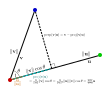
\includegraphics[width = 0.75\textwidth]{displacement_vector_proj_and_perp}
\end{center}

The projection \(\text{proj}(\mathbf{v}|\mathbf{u})\) is a multiple of \(\mathbf{u}\). The length of the projection is \(\|\mathbf{v}\|\cos\theta\) where \(\theta\) is the angle between \(\mathbf{u}\) and \(\mathbf{v}\). \(\|\mathbf{v}\|\cos\theta\) can be computed via:
\[\|\mathbf{v}\|\cos\theta = \frac{\|\mathbf{u}\|\|\mathbf{v}\|\cos\theta}{\|\mathbf{u}\|} = \frac{\mathbf{u} \bullet \mathbf{v}}{\|\mathbf{u}\|}\]
\(\frac{\mathbf{u}}{\|\mathbf{u}\|}\) is the normalization of \(\mathbf{u}\) that has the same direction as \(\mathbf{u}\) and a magnitude of \(1\). Multiplying \(\frac{\mathbf{u}}{\|\mathbf{u}\|}\) by the projection length gives the projection \(\text{proj}(\mathbf{v}|\mathbf{u})\):
\[\text{proj}(\mathbf{v}|\mathbf{u}) = (\|\mathbf{v}\|\cos\theta)\frac{\mathbf{u}}{\|\mathbf{u}\|} = \frac{\|\mathbf{u}\|\|\mathbf{v}\|\cos\theta}{\|\mathbf{u}\|^2}\mathbf{u} = \frac{\mathbf{u} \bullet \mathbf{v}}{\mathbf{u} \bullet \mathbf{u}}\mathbf{u}\]

One might ask the question: If \(\theta\) is obtuse, then the projection ``length" \(\|\mathbf{v}\|\cos\theta\) is negative. However in this case, the projection points in the opposite direction of \(\mathbf{u}\) so the negative sign does {\bf not} need to be removed.

The perpendicular component of \(\mathbf{v}\) remains when the projection is removed:
\[\text{perp}(\mathbf{v}|\mathbf{u}) = \mathbf{v} - \text{proj}(\mathbf{v}|\mathbf{u}) = \mathbf{v} - \frac{\mathbf{u} \bullet \mathbf{v}}{\mathbf{u} \bullet \mathbf{u}}\mathbf{u}\]

In summary, 
\[\text{proj}(\mathbf{v}|\mathbf{u}) = \frac{\mathbf{u} \bullet \mathbf{v}}{\mathbf{u} \bullet \mathbf{u}}\mathbf{u} \quad\text{and}\quad \text{perp}(\mathbf{v}|\mathbf{u}) = \mathbf{v} - \frac{\mathbf{u} \bullet \mathbf{v}}{\mathbf{u} \bullet \mathbf{u}}\mathbf{u}\]

If the magnitude of the projection is what is needed, then the magnitude is simply:
\[\|\text{proj}(\mathbf{v}|\mathbf{u})\| = \frac{|\mathbf{u} \bullet \mathbf{v}|}{\|\mathbf{u}\|}\]

If the magnitude of the perpendicular component is what is needed, then the magnitude can be computed from the magnitude of the projection via the Pythagorean theorem:
\[\|\text{perp}(\mathbf{v}|\mathbf{u})\| 
= \sqrt{\|\mathbf{v}\|^2 - \|\text{proj}(\mathbf{v}|\mathbf{u})\|^2} 
= \sqrt{\|\mathbf{v}\|^2 - \left(\frac{|\mathbf{u} \bullet \mathbf{v}|}{\|\mathbf{u}\|}\right)^2}
= \frac{\sqrt{\|\mathbf{u}\|^2\|\mathbf{v}\|^2 - (\mathbf{u} \bullet \mathbf{v})^2}}{\|\mathbf{u}\|}\]

If there is a line \(L\) that is parallel to \(\mathbf{u}\), and point \(P\) whose displacement from another point of the line is \(\mathbf{v}\), then \(\|\text{perp}(\mathbf{v}|\mathbf{u})\|\) is the shortest distance from line \(L\) to point \(P\).

It is easy to prove that \(\mathbf{u}\) and \(\text{perp}(\mathbf{v}|\mathbf{u})\) are perpendicular using the dot product: 
\[\mathbf{u} \bullet \text{perp}(\mathbf{v}|\mathbf{u}) = 
\mathbf{u} \bullet \left(\mathbf{v} - \frac{\mathbf{u} \bullet \mathbf{v}}{\mathbf{u} \bullet \mathbf{u}}\mathbf{u}\right) = 
\mathbf{u} \bullet \mathbf{v} - \frac{\mathbf{u} \bullet \mathbf{v}}{\mathbf{u} \bullet \mathbf{u}}(\mathbf{u} \bullet \mathbf{u}) = 
0\]

\textbf{Examples:}
\begin{itemize}
%%%%%%%%%%%%%%%%%%%%%
\item Let \(\mathbf{u} = \begin{bmatrix} 2 \\ -2 \\ 1 \end{bmatrix}\) and \(\mathbf{v} = \begin{bmatrix} -7 \\ 3 \\ 4 \end{bmatrix}\). \\
\(\mathbf{u} \bullet \mathbf{u} = \|\mathbf{u}\|^2 = 2^2 + (-2)^2 + 1^2 = 4 + 4 + 1 = 9\), \\
\(\mathbf{v} \bullet \mathbf{v} = \|\mathbf{v}\|^2 = (-7)^2 + 3^2 + 4^2 = 49 + 9 + 16 = 74\), and \\
\(\mathbf{u} \bullet \mathbf{v} = (2)(-7) + (-2)(3) + (1)(4) = -14 - 6 + 4 = -16\). Therefore:
\[\text{proj}(\mathbf{v}|\mathbf{u}) = \frac{\mathbf{u} \bullet \mathbf{v}}{\mathbf{u} \bullet \mathbf{u}}\mathbf{u} = \frac{-16}{9}\begin{bmatrix} 2 \\ -2 \\ 1 \end{bmatrix} = \begin{bmatrix} -32/9 \\ 32/9 \\ -16/9 \end{bmatrix}\]
and 
\[\text{perp}(\mathbf{v}|\mathbf{u}) = \mathbf{v} - \text{proj}(\mathbf{v}|\mathbf{u}) = \begin{bmatrix} -7 \\ 3 \\ 4 \end{bmatrix} - \begin{bmatrix} -32/9 \\ 32/9 \\ -16/9 \end{bmatrix} = \begin{bmatrix} -31/9 \\ -5/9 \\ 52/9 \end{bmatrix}\]
The magnitude of the projection is:
\[\|\text{proj}(\mathbf{v}|\mathbf{u})\| = \frac{|\mathbf{u} \bullet \mathbf{v}|}{\|\mathbf{u}\|} = \frac{|-16|}{3} = \frac{16}{3}\]
The magnitude of the perpendicular component is:
\[\|\text{perp}(\mathbf{v}|\mathbf{u})\| = \frac{\sqrt{\|\mathbf{u}\|^2\|\mathbf{v}\|^2 - (\mathbf{u} \bullet \mathbf{v})^2}}{\|\mathbf{u}\|} = \frac{\sqrt{(9)(74) - (-16)^2}}{3} = \frac{\sqrt{410}}{3}\]
%%%%%%%%%%%%%%%%%%%%%
\item Let \(\mathbf{u} = \begin{bmatrix} -3 \\ -2 \\ 1 \end{bmatrix}\) and \(\mathbf{v} = \begin{bmatrix} -1 \\ 5 \\ -7 \end{bmatrix}\). \\
\(\mathbf{u} \bullet \mathbf{u} = \|\mathbf{u}\|^2 = (-3)^2 + (-2)^2 + 1^2 = 9 + 4 + 1 = 14\), \\
\(\mathbf{v} \bullet \mathbf{v} = \|\mathbf{v}\|^2 = (-1)^2 + 5^2 + (-7)^2 = 1 + 25 + 49 = 75\), and \\ 
\(\mathbf{u} \bullet \mathbf{v} = (-3)(-1) + (-2)(5) + (1)(-7) = 3 - 10 - 7 = -14\). Therefore:
\[\text{proj}(\mathbf{v}|\mathbf{u}) = \frac{\mathbf{u} \bullet \mathbf{v}}{\mathbf{u} \bullet \mathbf{u}}\mathbf{u} = \frac{-14}{14}\begin{bmatrix} -3 \\ -2 \\ 1 \end{bmatrix} = \begin{bmatrix} 3 \\ 2 \\ -1 \end{bmatrix}\]
and 
\[\text{perp}(\mathbf{v}|\mathbf{u}) = \mathbf{v} - \text{proj}(\mathbf{v}|\mathbf{u}) = \begin{bmatrix} -1 \\ 5 \\ -7 \end{bmatrix} - \begin{bmatrix} 3 \\ 2 \\ -1 \end{bmatrix} = \begin{bmatrix} -4 \\ 3 \\ -6 \end{bmatrix}\]
The magnitude of the projection is:
\[\|\text{proj}(\mathbf{v}|\mathbf{u})\| = \frac{|\mathbf{u} \bullet \mathbf{v}|}{\|\mathbf{u}\|} = \frac{|-14|}{\sqrt{14}} = \sqrt{14}\]
The magnitude of the perpendicular component is:
\[\|\text{perp}(\mathbf{v}|\mathbf{u})\| = \frac{\sqrt{\|\mathbf{u}\|^2\|\mathbf{v}\|^2 - (\mathbf{u} \bullet \mathbf{v})^2}}{\|\mathbf{u}\|} = \frac{\sqrt{(14)(75) - (-14)^2}}{\sqrt{14}} = \frac{\sqrt{854}}{\sqrt{14}} = \sqrt{61}\]
%%%%%%%%%%%%%%%%%%%%%
\item Let \(\mathbf{u} = \begin{bmatrix} 1 \\ -3 \\ 0 \end{bmatrix}\) and \(\mathbf{v} = \begin{bmatrix} 5 \\ 2 \\ -7 \end{bmatrix}\). \\
\(\mathbf{u} \bullet \mathbf{u} = \|\mathbf{u}\|^2 = 1^2 + (-3)^2 + 0^2 = 1 + 9 + 0 = 10\), \\
\(\mathbf{v} \bullet \mathbf{v} = \|\mathbf{v}\|^2 = 5^2 + 2^2 + (-7)^2 = 25 + 4 + 49 = 78\), and \\
\(\mathbf{u} \bullet \mathbf{v} = (1)(5) + (-3)(2) + (0)(-7) = 5 - 6 + 0 = -1\). Therefore: 
\[\text{proj}(\mathbf{v}|\mathbf{u}) = \frac{\mathbf{u} \bullet \mathbf{v}}{\mathbf{u} \bullet \mathbf{u}}\mathbf{u} = \frac{-1}{10}\begin{bmatrix} 1 \\ -3 \\ 0 \end{bmatrix} = \begin{bmatrix} -1/10 \\ 3/10 \\ 0 \end{bmatrix}\]  
and 
\[\text{perp}(\mathbf{v}|\mathbf{u}) = \mathbf{v} - \text{proj}(\mathbf{v}|\mathbf{u}) = \begin{bmatrix} 5 \\ 2 \\ -7 \end{bmatrix} - \begin{bmatrix} -1/10 \\ 3/10 \\ 0 \end{bmatrix} = \begin{bmatrix} 51/10 \\ 17/10 \\ -7 \end{bmatrix}\]
The magnitude of the projection is:
\[\|\text{proj}(\mathbf{v}|\mathbf{u})\| = \frac{|\mathbf{u} \bullet \mathbf{v}|}{\|\mathbf{u}\|} = \frac{|-1|}{\sqrt{10}} = \frac{1}{\sqrt{10}}\]
The magnitude of the perpendicular component is:
\[\|\text{perp}(\mathbf{v}|\mathbf{u})\| = \frac{\sqrt{\|\mathbf{u}\|^2\|\mathbf{v}\|^2 - (\mathbf{u} \bullet \mathbf{v})^2}}{\|\mathbf{u}\|} = \frac{\sqrt{(10)(78) - (-1)^2}}{\sqrt{10}} = \frac{\sqrt{779}}{\sqrt{10}} = \sqrt{\frac{779}{10}}\]
\end{itemize}

%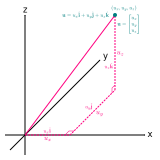
\includegraphics[width = \textwidth]{3_vector}


\end{document}










